\documentclass[a4paper, 11pt]{article}
\usepackage{lipsum} %This package just generates Lorem Ipsum filler text. 
\usepackage{fullpage} % changes the margin
\usepackage{mathpazo}
\usepackage{multicol}
\usepackage{graphicx}
\usepackage{enumerate}
\usepackage{amsmath,amsfonts,amsthm} % Math packages
\usepackage{listings}
\usepackage{fontspec}

\usepackage{matlab-prettifier}

\begin{document}
%Header-Make sure you update this information!!!!
\noindent
\large\textbf{Homework 4} \hfill \textbf{Hongyu Yan (516030910595)} \\
\normalsize {\bf CS 259 Numerical Methods for Data Science} \hfill ACM Class, Zhiyuan College, SJTU\\
Prof.~{\bf David Bindel} \hfill Due Date: June 26th, 2018\\
TA.~{\bf Yurong You, Xinran Zhu} \hfill Submit Date: \today

\section*{Problem 1}

\begin{figure}[htbp]
\centering
	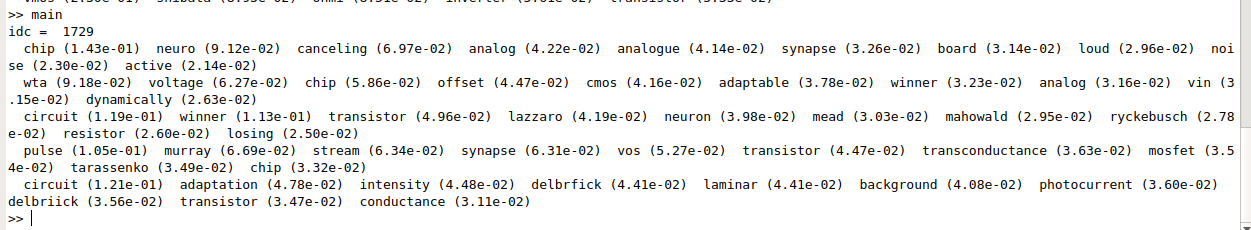
\includegraphics[scale=0.4]{result.png}
	\caption{Result}
	\label{fig1}
\end{figure}
The result shows that the most relevant articles may not have "circuit" as top words.
It seems that "circuit" may refer to biological neural network, which means the documents'
top words may contain "synapse", "neuro" etc.
It may also refer to electronics related themes, which means the documents' top words may be "chip", "pulse" etc.

Here is my code.

\begin{lstlisting}[language = Matlab, numbers=left,   
  numberstyle=\tiny,keywordstyle=\color{blue!70},  
  commentstyle=\color{red!50!green!50!blue!50},frame=shadowbox,  
  rulesepcolor=\color{red!20!green!20!blue!20},basicstyle=\ttfamily,
  tabsize=2]

[W, vocab] = load_docword('.', 'nips');
[WW, Dtf, Didf] = tf_idf(W);


[U, S, V] = svds(WW, 20);
new_WW = U * S * V';

idc = 0;
for i = 1:length(vocab)
	if strcmp(vocab{i}, 'circuit')
		idc = i
	end
end

score = new_WW(:, idc);
[v, idx] = sort(score, 'descend');

num_doc = 5;
num_word = 10;
for i = 1:num_doc
	show_top_words(WW(idx(i), :), vocab, num_word);
end

\end{lstlisting}
\end{document}
